\section*{Related work}\label{ch:ch2label}

\subsection*{Physically based differentiable rendering}

Until now, the researchers have been focusing on differentiable light transport integral.
These include solving geometric discontinuity problem on the integral\cite{li2018differentiable, loubet2019reparameterizing, zhang2020path}. In all these works, the derivatives with respect to scene parameters are calculated by automatic differentiation. Especially, by reverse-mode differentiation the derivatives with respect to multiple scene parameters are computed at once. Though multi-derivatives are concurrently possible, we need another technique about some parameters or joint optimization problem, due to the local minima.

\subsection*{Laplacian smooth gradient descent}

Stochastic gradient descent (SGD) is the workhorse in modern optimization technique. However, due to the variance, descent behavior sometimes shows the result that cannot overcome being stuck in local minima. 

Osher et al\cite{osher2018laplacian} suggested the method to take larger steps than original SGD, which is enabled by simply multiplying gradient with discrete one-dimensional Laplacian.

\begin{align}{\label{eq:1}}
	x \leftarrow x - \eta (I + \lambda L)^{-p} {\frac{\partial \Phi}{\partial x}}
\end{align}

\subsection*{Laplacian smoothing in computer graphics}

In geometry processing, the Laplacian operator has been the key tool for solving many kinds of geometry problem. Though there may be many references about Laplacian properties, discrete Laplacians are enough in here.

\begin{figure}[!h]
    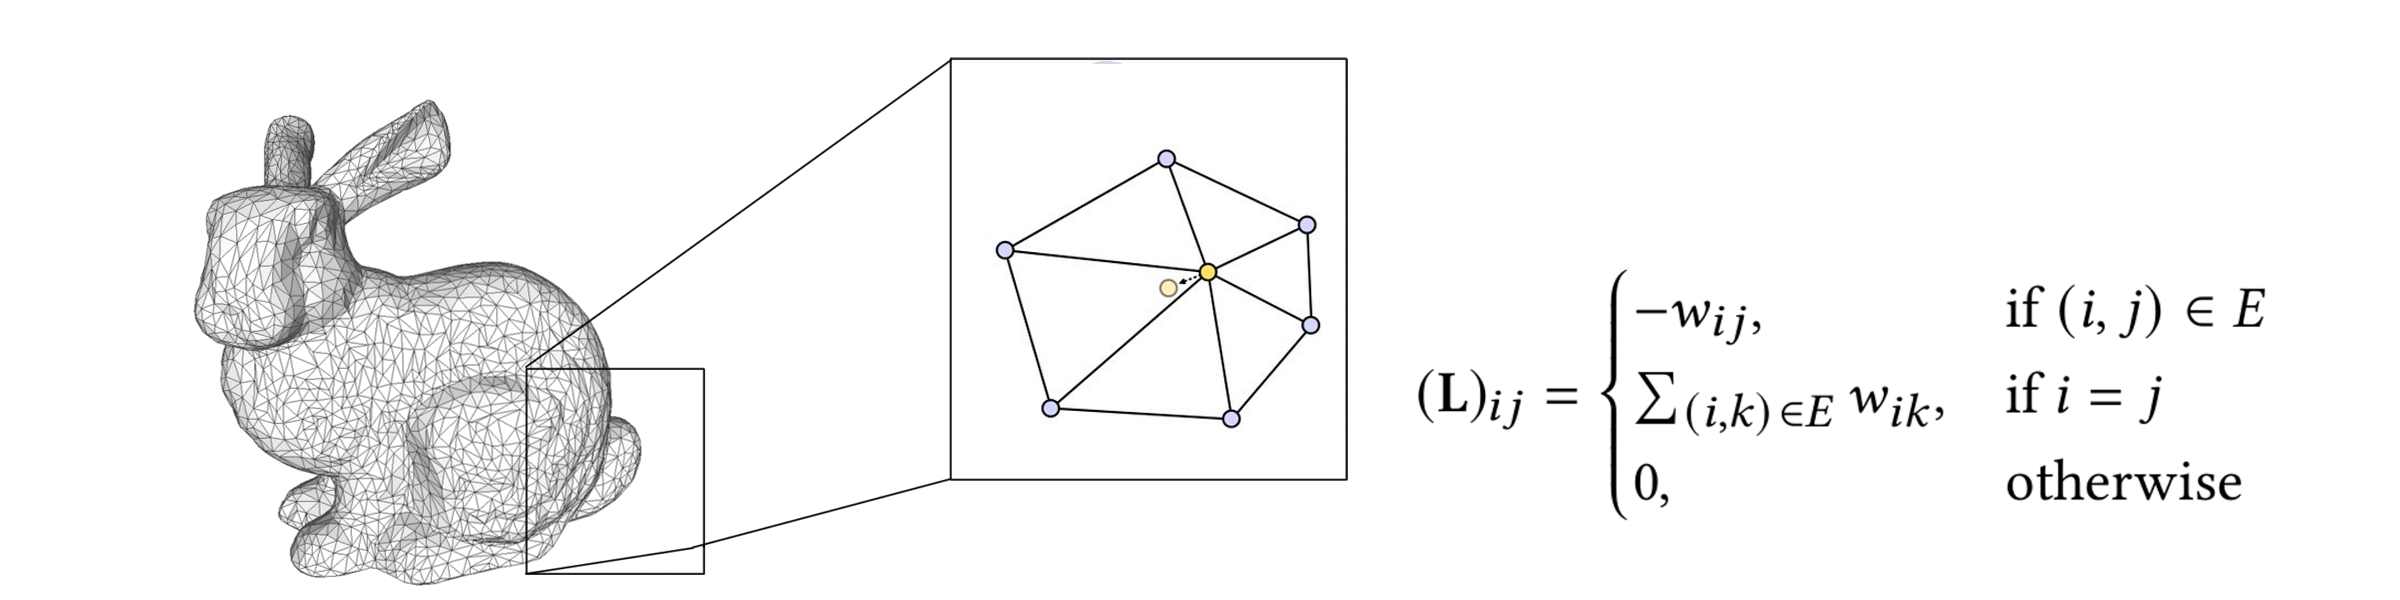
\includegraphics[width=\textwidth]{figures/related-work-1.png}
    \caption{Discrete Laplacian on Mesh}
    \label{fig:discreteLaplacian}
\end{figure}

% Discrete Laplacian\ref{fig:discreteLaplacian} some depiction
% Generally, cotangent matrix, in real combination, 
% this is combined with mesh massmatrix 

Nicolet et al\cite{Nicolet2021Large} propose the application method of Laplacian smooth to mesh optimizing on differentiable rendering. The authors convert the iterative update form to fit in geometry processing.
From the equation\ref{eq:1}, the $L$ is calculated from discrete Laplacian on mesh. This form can be interpreted as Osher's method\cite{osher2018laplacian}. Otherwise, from the point of view of geometry processing, this can be Sobolev preconditioned form, or for easy understanding
filtering noisy vertices from the target mesh before gradient descent step every iteration.